% Copyright (c) 2023 Ludovic Lars
% This work is licensed under the CC BY-NC-SA 4.0 International License

\chapter{Le passage à l'échelle}
\label{ch:scalabilite}
\label{enotezch:14}

% Scalabilité
\lettrine[]{L}a scalabilité, calque de l'anglais \eng{scalability}, aussi appelée extensibilité, désigne la capacité d'un système à passer à l'échelle, c'est-à-dire à continuer de fonctionner de manière équivalente à mesure que le nombre d'utilisateurs augmente. Dans un système géré de manière centralisée, cette capacité est assurée par l'apport de matériel informatique, soit en ajoutant de la puissance de calcul à l'infrastructure existante (passage à l'échelle vertical), soit en multipliant les instances de l'infrastructure pour partager le traitement des requêtes (passage à l'échelle horizontal). La scalabilité dépend par conséquent du niveau de prévision de l'entité qui s'occupe du système.

% Système distribué, Bitcoin
Dans le cas d'un système distribué, qui a un comportement différent, la scalabilité se rapporte à quelque chose de plus compliqué. L'ajout de matériel ne suffit pas~: il faut également que les propriétés dudit système se conservent avec la hausse de l'activité. Dans le cas de Bitcoin, ce problème est particulièrement ardu, car toute montée en charge affecte durablement les nœuds du réseau, en raison de la nécessité de partage de la chaîne de blocs intégrale. En substance, le système ne passe pas à l'échelle, ou très peu.

% Débat sur la scalabilité
Ce problème de scalabilité de Bitcoin a été une préoccupation majeure de la communauté, à tel point qu'il a provoqué un véritable conflit ouvert entre 2015 et 2017~: la fameuse guerre des blocs que nous avons décrite dans le chapitre~\ref{ch:clivages}. Certains pensaient qu'augmenter la taille des blocs suffiraient à gérer la demande sans altérer l'offre, tandis que d'autres imaginaient que les solutions de surcouche comme le réseau Lightning seraient assez efficaces pour traiter tous les transferts. Ce chapitre a pour objectif de faire un tour d'horizon de la situation et de proposer une troisième voie.

\section*{L'absence de scalabilité du système} % Non-scalabilité
\addcontentsline{toc}{section}{L'absence de scalabilité du système}

% Vérification de toutes mes transactions
La conception originelle de Bitcoin repose sur un principe simple~: obtenir et vérifier l'intégralité des transactions dans le but de s'assurer qu'il n'y a pas de double dépense. Comme l'écrivait Satoshi Nakamoto dans le livre blanc, «~la seule façon de confirmer l'absence d'une transaction est d'être au courant de toutes les transactions\footnote{Satoshi Nakamoto, \eng{Bitcoin: A Peer-to-Peer Electronic Cash System}, 31 octobre 2008.}~». De ce fait, pour disposer d'une sécurité maximale, chaque nœud doit, en principe, entretenir une version complète de la chaîne de blocs.

% Message de James A. Donald
Dès les origines, ce fonctionnement particulier a naturellement amené la question de la montée en charge du système. Lorsque Satoshi Nakamoto a présenté sa découverte sur la liste de diffusion dédiée à la cryptographie de Metzdowd.com le 31 octobre 2008, la première réponse qu'il a reçue concernait ainsi ce problème. Cette réponse était celle de l'ancien cypherpunk James A. Donald le 2 novembre, qui écrivait~:

\begin{quote}
«~Nous avons vraiment, vraiment besoin d'un tel système, mais d'après ce que je comprends de votre proposition, il ne semble pas pouvoir s'adapter à la taille requise.

Pour que des jetons de preuve de travail transférables aient de la valeur, ils doivent avoir une valeur monétaire. Pour avoir une valeur monétaire, ils doivent être transférés au sein d'un très grand réseau --- par exemple un réseau d'échange de fichiers semblable à bittorrent.

Pour détecter et rejeter un événement de double dépense dans un délai convenable, il faut disposer de la plupart des transactions passées des pièces impliquées dans la transaction, ce qui, mis en œuvre naïvement, exige que chaque pair dispose de la plupart des transactions passées, ou de la plupart des transactions passées qui ont eu lieu récemment. Si des centaines de millions de personnes effectuent des transactions, cela représente beaucoup de bande passante --- chacun doit avoir connaissance de toutes les transactions ou d'une partie substantielle de celles-ci\footnote{James A. Donald, \eng{Re: Bitcoin P2P e-cash paper}, \wtime{02/11/2008, 23:46:23 UTC}~: \url{https://www.metzdowd.com/pipermail/cryptography/2008-November/014814.html}.}.~»
\end{quote} % "We very, very much need such a system, but the way I understand your proposal, it does not seem to scale to the required size.
%
% For transferable proof of work tokens to have value, they must have monetary value. To have monetary value, they must be transferred within a very large network - for example a file trading network akin to bittorrent.
%
% To detect and reject a double spending event in a timely manner, one must have most past transactions of the coins in the transaction, which,  naively implemented, requires each peer to have most past transactions, or most past transactions that occurred recently. If hundreds of millions of people are doing transactions, that is a lot of bandwidth - each must know all, or a substantial part thereof."

% Manque de scalabilité, compromis entre utilité et sécurité
James A. Donald mettait par là en valeur le manque de scalabilité de Bitcoin. Pour tout système donné, une augmentation de volume transactionnel accroît le nombre de transactions à obtenir et à traiter. Cet accroissement rend plus difficile de faire fonctionner un nœud, ce qui peut affecter la décentralisation du réseau et donc la sécurité. De ce fait, il existe toujours un compromis entre l'utilité et la sécurité du système, ou pour mieux le dire, entre la facilité de transaction et la facilité de vérification\pagenote{«~entre la facilité de transaction et la facilité de vérification~»~: Sosthène, \emph{Apologie des petits blocs}, 2 août 2018~: \url{https://www.sosthene.net/apologie-petits-blocs/}.}.

% Limite de capacité transactionnelle, taille limite des blocs
Ce compromis se manifeste généralement par une limite de capacité transactionnelle\pagenote{«~Ce compromis se manifeste généralement par une limite de capacité transactionnelle~»~: Dans le cas où elle n'est définie nulle part, cette limite est de toute manière inférieure à la limite de marché du mineur le plus efficace, car aucun mineur économiquement rationnel ne traiterait de transaction gratuitement.}, décrite par les règles de consensus (limite explicite) ou, plus rarement, par les règles de réseau (limite implicite). La limite de capacité transactionnelle était originellement décrite comme une taille limite des blocs, qui interdisait aux mineurs de créer des blocs plus grands qu'une certaine taille. Dans le prototype, cette taille était définie implicitement par la taille maximale des messages du protocole de transmission, c'est-à-dire 32~Mio. Puis, une limite explicite de 1 mégaoctet (1~Mo) a été ajoutée par Satoshi Nakamoto en septembre 2010 par le biais de la constante \longstring{MAX\_BLOCK\_SIZE}, sans annonce publique de sa part, dans le but d'éviter les attaques par déni de service. Cette taille correspondait, pour un réseau tournant à plein régime, à un volume théorique de 4,5 transactions classiques par seconde, ce qui se ramenait plutôt à 3 transactions par seconde en pratique. % Théorique. P2PKH : 1e2s, 226o (max) ; 2e2s, 374o (max). #tx = 1e6 / (taille_tx * 600) : 1e2s, 7.37 tx/s ; 2e2s, 4,46 tx/s. / Pratique : https://www.blockchain.com/explorer/charts/transactions-per-second

% Poids limite des blocs
Avec l'intégration de SegWit dans la version principale de Bitcoin en août 2017, cette limitation est devenue un poids limite des blocs. Cette nouvelle métrique donnait une importance plus grande de la taille de base par rapport à la taille du témoin dans le calcul de la mesure du bloc, modifiant également la façon dont comptaient les mineurs pour ajouter les transactions au bloc. Cette modification était une augmentation effective de la capacité transactionnelle du protocole, portant le volume autorisé de transactions à 8 transactions par seconde en théorie, et à 4,5 transactions par seconde en pratique. % Théorique. P2WPKH : 1e2s, 223o, 562 wu (max) ; 2e2s, 372o, 834 wu (max). #tx = 4e6 / (poids_tx * 600) : 1e2s, 11.86 tx/s ; 2e2s, 7.99 tx/s. / Pratique : https://www.blockchain.com/explorer/charts/transactions-per-second

% Rareté de l'espace de bloc
L'existence d'une limite de capacité transactionnelle engendre nécessairement une rareté de l'espace de bloc. Si elle est fixe, elle rend l'offre par essence inélastique. Ainsi, une forte demande pour l'espace de bloc fait, par effet d'enchère, augmenter le prix pour l'inclusion, c'est-à-dire les frais de transaction. Le marché des frais est stimulé par cette limite rigide au lieu de rester à son niveau naturel, à savoir celui du coût d'inclusion par défaut des mineurs.

% Plancher d'utilité
Par son effet sur le niveau des frais, la limite crée un plancher d'utilité, c'est-à-dire un niveau de valeur en deçà duquel le transfert et la détention ne sont pas considérés comme rentables par les utilisateurs. En effet, les mineurs sont amenés à rejeter les transactions qui ne paient pas un taux de frais suffisant par rapport à leur taille. De ce fait, l'utilité d'une transaction peut être estimée insuffisante par son auteur au regard du niveau de frais moyen de la chaîne, auquel cas elle n'a pas lieu. Si une personne désire acheter un café pour 2~\$ en BTC, mais que les frais usuels sont de 1~\$, cette personne passera vite son chemin. De manière générale, les cas d'utilisation requérant des frais «~faibles~» sont chassés de la chaîne, à l'instar du service de jeu d'argent SatoshiDICE, qui a dû cesser ses activités sur BTC en 2017 suite à l'augmentation des frais.

% Impact de la limite de capacité transactionnelles sur la décentralisation
La limite de capacité transactionnelle a pour vertu de garantir que le coût d'utilisation d'un nœud reste bas. Elle agit ainsi sur la décentralisation \emph{potentielle} du réseau. En effet, contrairement au matériel minier, le coût lié à la vérification n'est pas compensé par un revenu proportionnel, de sorte qu'il atteint tout le monde de la même manière. Les opérateurs de nœud les moins bien équipés ne peuvent pas matériellement suivre le rythme, ce qui affecte la facilité du réseau à se décentraliser \emph{effectivement}. % Minage : machines de hachage et les mécanismes de refroidissement associés

% Rôle dans le modèle de sécurité
L'influence sur la décentralisation potentielle concerne à la fois le minage et le commerce en empêchant les plus petits acteurs de pouvoir réaliser ces activités à leur échelle. La centralisation du minage augmente le risque de censure, tandis que la centralisation du commerce augmente le risque d'altération du protocole, et donc le risque d'inflation. C'est pourquoi la limite de capacité transactionnelle joue un rôle majeur dans le modèle de sécurité~: moins cette limite est élevée, plus la sécurité \emph{potentielle} du système est grande.

% Limite arbitraire liée à l'interprétation subjective des commerçants
La limite de capacité transactionnelle est déterminée de manière subjective par les commerçants, en fonction de leur \emph{perception de la menace} et de leur \emph{utilisation personnelle} de la chaîne. Il n'existe pas de limite de taille des blocs idéale~: il n'y a que des êtres humains qui calculent un risque par rapport à une éventuelle récompense. On peut tenter d'établir une moyenne pour estimer une limite qui correspond à une utilisation donnée, mais cette estimation serait au mieux imparfaite.

% Plafond d'utilité
Par son effet sur la décentralisation, la limite crée un plafond d'utilité, c'est-à-dire un niveau de valeur au-delà duquel le transfert et la détention sont considérés trop risqués pour la sécurité effective du système. En effet, aucune sécurité n'étant absolue, le transfert et la détention d'une certaine valeur peut ne plus bénéficier suffisamment de la protection apportée par le réseau. Par exemple, recevoir ou conserver l'équivalent de plusieurs millions de dollars sur la chaîne de Bitcoin SV est, c'est le moins qu'on puisse dire, imprudent.

% Plage de valeurs
Le plancher d'utilité (induit par l'action négative de la limite sur l'espace de bloc) et le plafond d'utilité (induit par l'action positive de la limite sur la sécurité) ont pour effet de borner une plage de valeurs en dehors de laquelle le transfert et la détention ne sont plus pertinents\footnote{Voir Eric Voskuil, «~Propriété du seuil d'utilité~», in \emph{Cryptoéconomie~: Principes fondamentaux de Bitcoin}, Amazon KDP, 2022, pp.~317--318.}. C'est l'existence de cette plage de valeurs qui entraîne l'apparition de substituts à un système donné.

% Non-scalabilité
L'arrivée de nouveaux utilisateurs et l'augmentation subséquente de la demande pour l'espace de blocs rehaussent le plancher d'utilité. Toute montée en charge du système en modifie les caractéristiques. Par conséquent, tout système Bitcoin est en substance non scalable, au sens premier du terme. Il existe cependant des méthodes pour contourner cette absence de scalabilité.

\section*{L'amélioration de l'efficacité de base}
\addcontentsline{toc}{section}{L'amélioration de l'efficacité de base}

% Augmentation progressive de la taille limite des blocs
La première proposition vis-à-vis du passage à l'échelle a été d'augmenter progressivement la limite de taille des blocs dans le but d'accompagner l'accroissement de l'activité\footnote{Parmi les versions alternatives de Bitcoin, la voie de l'augmentation progressive de la taille limite des blocs a été choisie par Bitcoin Cash, qui prévoit d'intégrer un algorithme permettant de gérer cette augmentation automatiquement. Voir bitcoincashautist, \eng{CHIP-2023-04: Adaptive Blocksize Limit Algorithm for Bitcoin Cash}, 2 septembre 2023~: \url{https://gitlab.com/0353F40E/ebaa/-/blob/f4edacd134103a7e232740463a5f26379bf90f18/README.md}.

Elle a également été favorisée de manière plus conservatrice par Monero, qui possède une taille de bloc dynamique basée sur un mécanisme de pénalité pour compenser les \emph{excès} par rapport à la normale. Voir SerHack, \eng{Mastering Monero: The Future of Private Transactions}, Amazon KDP, 2018, pp.~136--139.}\pagenote{«~augmenter progressivement la limite de taille des blocs dans le but d'accompagner l'accroissement de l'activité~»~: Dans Monero, la pénalité ($P$) liée à la taille d'un bloc ($B$) est calculée à partir la taille médiane des 100 derniers blocs ($M$) et la subvention de base ($R$) qui est de 0,6~XMR par bloc depuis 2022. Si $B < M_0 = 300~\mathrm{ko}$, alors $P = 0$. Sinon~:
\[
P = R  \left( \frac{B}{M} - 1 \right)^2~.
\]
La taille du bloc ne peut pas dépasser $2 M$ (taille qui correspond à une pénalité maximale).}. C'était la solution soutenue par Satoshi Nakamoto\pagenote{«~C'était la solution soutenue par Satoshi Nakamoto~»~: Satoshi Nakamoto, \eng{Re: [PATCH] increase block size limit}, \wtime{04/10/2010 19:48:40 UTC}~: \url{https://bitcointalk.org/index.php?topic=1347.msg15366\#msg15366}.}, comme en témoigne sa première réaction à la réponse de James A. Donald le 3 novembre 2008~:

\begin{quote}
«~La bande passante n'est peut-être pas aussi prohibitive que vous le pensez. Une transaction typique est d'environ 400 octets (la cryptographie sur les courbes elliptiques est agréablement compacte). Chaque transaction doit être diffusée deux fois, soit 1 Ko par transaction. Visa a traité 37 milliards de transactions au cours de l'année 2008, soit une moyenne de 100 millions de transactions par jour. Un tel nombre de transactions nécessiterait 100 Go de bande passante, soit la taille de 12 DVD ou de 2 films en qualité HD, ou encore environ 18~\$ de bande passante au prix actuel. Si le réseau devait atteindre cette taille, cela prendrait plusieurs années, et d'ici là, l'envoi de 2 films en HD sur Internet ne semblera probablement pas être un gros problème\footnote{Satoshi Nakamoto, \eng{Re: Bitcoin P2P e-cash paper}, \wtime{03/11/2008, 01:37:43 UTC}~: \url{https://www.metzdowd.com/pipermail/cryptography/2008-November/014815.html}.}.~»
\end{quote} % "The bandwidth might not be as prohibitive as you think.  A typical transaction would be about 400 bytes (ECC is nicely compact).  Each transaction has to be broadcast twice, so lets say 1KB per transaction.  Visa processed 37 billion transactions in FY2008, or an average of 100 million transactions per day.  That many transactions would take 100GB of bandwidth, or the size of 12 DVD or 2 HD quality movies, or about $18 worth of bandwidth at current prices. If the network were to get that big, it would take several years, and by then, sending 2 HD movies over the Internet would probably not seem like a big deal."

% Satoshi avait tort
La vision de Satoshi était cependant bien trop optimiste. D'une part, il ne voyait pas la centralisation du minage comme un problème existentiel, prévoyant dès le début que la puissance de calcul du réseau reposerait sur des «~fermes de serveurs composées de matériel spécialisé~». D'autre part, il pensait que la vérification de paiement simplifiée suffirait, ne tenant pas compte de ses défauts de fiabilité et de confidentialité, ni de son incapacité à exercer un pouvoir sur la détermination des règles de consensus. Le plan de Satoshi était donc faillible sans pour autant être entièrement mauvais.

% Facteurs limitants
Le fonctionnement d'un nœud dépend d'un certain nombre de charges. Les principales sont le stockage sur disque dur (HDD) pour l'historique (chaîne de blocs), le stockage en mémoire flash (SSD) pour l'état (ensemble des UTXO), le stockage en mémoire vive (barrette de RAM) pour la réserve des transactions non confirmées (mempool) et la réserve des blocs orphelins, le maintien d'une bande passante (ou débit binaire, usuellement exprimé en Mbit/s) permettant de recevoir et d'envoyer les blocs et les transactions, et le calcul du processeur (CPU) pour la vérification des données et notamment des signatures. Faire diminuer le coût d'un nœud consiste ainsi à réduire l'une de ces charges.

% Optimisation
Même si l'augmentation naïve de la taille limite des blocs ne constitue pas en soi une méthode de scalabilité, il s'avère qu'elle peut être compensée par le progrès technique provenant de l'optimisation logicielle, matérielle ou algorithmique. Premièrement, les performances du logiciel (pour un ensemble donné de règles de consensus) peuvent être améliorées, et il s'agit même de l'une des tâches de base de l'équipe de Bitcoin Core\footnote{Voir par exemple l'article de Jameson Lopp sur l'évolution de la performance de Bitcoin Core dans lequel décrit comment la première synchronisation sur sa machine s'est améliorée au cours des années. -- Jameson Lopp, \eng{Bitcoin Core Performance Evolution}, 5 mars 2022~: \url{https://blog.lopp.net/bitcoin-core-performance-evolution/}.}. Deuxièmement, le matériel informatique peut être rendu plus efficace, certains composants devenant progressivement moins coûteux (loi de Moore\footnote{La loi de Moore est une conjecture énoncée par Gordon E. Moore en 1965 ayant postulé que la complexité des semi-conducteurs doublait chaque année. Cette loi était citée par Satoshi Nakamoto dans le livre blanc, qui écrivait~: «~La loi de Moore prédisant une croissance actuelle de 1,2 Go par an, le stockage ne devrait pas poser de problème même si les entêtes de blocs doivent être conservés en mémoire.~» -- Satoshi Nakamoto, \eng{Bitcoin: A Peer-to-Peer Electronic Cash System}, 31 octobre 2008.}). Troisièmement, le protocole peut lui-même être perfectionné au niveau algorithmique, par la découverte et l'adoption de nouvelles techniques plus efficaces~: c'est par exemple le cas de l'algorithme de signature de Schnorr qui produit des signatures plus compactes qu'ECDSA (40~octets au lieu de 72), ou bien des bulletproofs qui rendent les preuves de portée des Confidential Transactions beaucoup moins volumineuses.

% Modifier le comportement du système
Au-delà de ces optimisations, il n'existe pas de manière d'augmenter le volume transactionnel de la chaîne sans faire de compromis au niveau du modèle de Bitcoin. La solution consiste ainsi à modifier le comportement du système, de telle manière qu'il n'affecte pas trop le modèle de sécurité. Plusieurs facteurs peuvent ainsi être optimisés, dont la taille de la chaîne à conserver, l'\eng{Initial Block Download} (IDB) et la taille de l'ensemble des UTXO.

% Taille de la chaîne
D'abord, on peut choisir de supprimer les blocs les plus anciens une fois qu'on les a vérifiés. On conserve simplement la chaîne des entêtes, l'état du réseau, ainsi que les blocs les plus récents afin de pouvoir rejoindre le consensus dans le cas d'une recoordination profonde. Cette méthode est appelée l'élagage ou \eng{pruning}.

% IBD
Mais cette méthode n'enlève pas la charge de l'IBD, c'est-à-dire le processus de téléchargement et de vérification de la chaîne de blocs jusqu'à sa hauteur actuelle. Pour ce faire, on peut procéder à diverses techniques plus ou moins risquées. La première est la supposition de validité des signatures, basée sur le paramètre \texttt{assumevalid}, qui a été introduite dans Bitcoin Core en 2017\footnote{Bitcoin Core, \eng{Bitcoin Core 0.14.0}, 8 mars 2017~: \url{https://bitcoincore.org/en/2017/03/08/release-0.14.0/\#assumed-valid-blocks}.}, et qui consiste à sauter la vérification des signatures jusqu'à un bloc d'empreinte donnée, faisant gagner beaucoup de temps dans la synchronisation initiale. Cette méthode n'est pas un point de contrôle (elle n'impose pas au bloc d'exister) et le risque qu'elle comporte est minime. La deuxième technique est AssumeUTXO, qui a été proposée en 2019 par James O'Beirne et est toujours en développement\footnote{James O'Beirne, \eng{AssumeUTXO Proposal}, 24 avril 2019~: \url{https://github.com/jamesob/assumeutxo-docs/tree/2019-04-proposal/proposal}.}, et qui implique de supposer valide un ensemble des UTXO donné (identifié par son empreinte) à une hauteur de bloc déterminée~: l'opérateur de nœud télécharge la sauvegarde de l'ensemble des UTXO auprès d'un tiers et débute la synchronisation initiale à partir de celui-ci, remettant à plus tard (ou ignorant complètement) le téléchargement et la vérification des blocs précédents. Cette méthode présente un défaut de vérification (au moins temporaire) de sorte que l'opérateur est exposé à la tromperie, mais le risque est considéré comme acceptable\pagenote{«~Cette méthode présente un défaut de vérification (au moins temporaire) de sorte que l'opérateur est exposé à la tromperie, mais le risque est considéré comme acceptable~»~: Les risques liées à AssumeValid et à AssumeUTXO sont discutés dans le chapitre~5 de l'ouvrage \eng{Bitcoin: A Work in Progress} de Sjors Provoost publié en 2022.}. Il existe également une troisième technique plus radicale, l'engagement des UTXO (ou \eng{UTXO commitments}), qui est un soft fork obligeant les mineurs à ajouter l'empreinte de l'ensemble des UTXO dans le bloc\footnote{Mark Friedenbach, \eng{[soft fork] Block v3: miner commitments with compact proofs}, 28 mars 2014~: \url{https://github.com/bitcoin/bitcoin/pull/3977}~; Pieter Wuille, \eng{[bitcoin-dev] Rolling UTXO set hashes}, \wtime{15/05/2017 20:01:14 UTC}~: \url{https://lists.linuxfoundation.org/pipermail/bitcoin-dev/2017-May/014337.html}.}~: cet engagement permettrait de disposer d'une source bien plus fiable pour télécharger la sauvegarde à partir de laquelle commencer la synchronisation.

% UTXO set
Ensuite, au-delà de l'IBD, reste le problème de la taille de l'ensemble des UTXO, qui est l'un des facteurs limitants les plus importants. La première idée pour réduire cette taille est une proposition de Cory Fields appelée UHS (pour \eng{UTXO Hash Set}) qui consiste uniquement à stocker les empreintes (\eng{hashes}) des UTXO individuelles\footnote{Cory Fields, \eng{UHS: Full-node security without maintaining a full UTXO set}, \wtime{16/05/2018 16:36:35 UTC}~: \url{https://lists.linuxfoundation.org/pipermail/bitcoin-dev/2018-May/015967.html}.}. La deuxième idée est de se servir d'accumulateurs cryptographiques, comme l'a fait Thaddeus Dryja avec sa proposition nommée Utreexo, qui implique de regrouper les UTXO dans des arbres de Merkle afin de condenser l'ensemble à conserver en mémoire, au prix d'un compromis sur la bande passante\footnote{Thaddeus Dryja, \eng{Utreexo: A dynamic hash-based accumulator optimized for the Bitcoin UTXO set}, 6 juin 2019~: \url{https://eprint.iacr.org/2019/611.pdf}.}. % prononcée «~\eng{U-Tree-X-O}~»

% CISA : Cross-Input Signature Aggregation.

% Sharding
Enfin, on peut également choisir d'éclater le minage et la vérification des transactions en séparant l'historique et l'état du système en plusieurs fragments, qui sont chacun soutenus par une partie (variable) du réseau. C'est ce qu'on appelle le partitionnement ou \eng{sharding}. C'était l'idée derrière l'utilisation d'un arbre préfixe de Merkle-Patricia (aussi appelé arbre Merklix) vaguement envisagée par les développeurs de Bitcoin Cash\pagenote{«~vaguement envisagée par les développeurs de Bitcoin Cash~»~: Amaury Séchet, \eng{Using Merklix tree to shard block validation}, 6 novembre 2016~: \url{http://www.deadalnix.me/2016/11/06/using-merklix-tree-to-shard-block-validation}, archive~: \url{https://web.archive.org/web/20170716220359/https://www.deadalnix.me/2016/11/06/using-merklix-tree-to-shard-block-validation/}~; Joannes Vermorel, Amaury Séchet, Shammah Chancellor, Jason Cox, \eng{Merklix tree for Bitcoin}, juillet 2018~: \url{https://blog.vermorel.com/pdf/merklix-tree-for-bitcoin-2018-07.pdf}.}, ou le \eng{danksharding} qui pourrait être implémenté dans Ethereum\pagenote{«~le danksharding qui pourrait être implémenté dans Ethereum~»~: \url{https://ethereum.org/en/roadmap/danksharding/}.}. Cependant, il s'agit là d'une modification importante du protocole qui pourrait ne jamais être implémentée dans une version de Bitcoin.

%
Ces propositions sont des compromis se faisant au niveau de la chaîne qui affectent souvent le système dans son entièreté. Toutefois, il est également possible de faire un compromis différent, au niveau des pièces individuelles, par l'utilisation de banques et, surtout, de surcouches.

% Toutefois, on peut considérer que le compromis réalisé n'est pas à même de couvrir l'ensemble des plages de valeurs pour traiter l'intégralité de la demande transactionnelle existante...

\section*{Les banques et les surcouches}
\addcontentsline{toc}{section}{Les banques et les surcouches}

Les autres propositions généralement citées comme alternatives à l'augmentation de la taille des blocs sont des solutions consistant à ne pas réaliser tous les transferts sur la chaîne, mais à en déporter les plus petits ailleurs, ceux-ci étant «~regroupés~» dans des transactions plus grosses. La chaîne est alors utilisée pour régler les dettes, contractées de manière analogique (contrat juridique) ou numérique (contrat autonome). Cela consiste à considérer le protocole comme un protocole de règlement.

% La première application dépositaire de ce type était MyBitcoin (2010 - 2011), une interface web permettant un usage facile et serein de Bitcoin, y compris sur mobile.

% Modèle de banque libre
La première manière de faire est de réintroduire de la confiance dans le système en contractant des obligations de manière traditionnelle, auprès de ce que nous appellerons ici des banques. Les banques en question peuvent émettre une monnaie représentative en gardant l'intégralité des fonds, ou bien offrir du crédit en ne conservant que des réserves fractionnaires. L'utilisation de la chaîne sert au règlement entre les banques, qui assure le transfert de fonds entre leurs clients. C'est en somme le modèle de la banque libre promu par George Selgin et Larry White dans les années 1990.

% Hal Finney
Cette première conception a été défendue par Hal Finney, qui avait connaissance des travaux de Selgin et de White, comme nous l'avons vu dans le chapitre~\ref{ch:cybermonnaie}. Le 30 décembre 2010, il faisait ainsi l'apologie d'un modèle de banque libre basé sur le bitcoin~:

\begin{quote}
«~En fait, il existe une très bonne raison pour que les banques basées sur Bitcoin existent et émettent leur propre monnaie numérique, convertible en bitcoin. Bitcoin lui-même ne peut pas passer à l'échelle pour que chaque transaction financière dans le monde soit diffusée publiquement et incluse dans la chaîne de blocs. Il doit y avoir un niveau secondaire de systèmes de paiement, plus léger et plus efficace. [...] Les banques basées sur Bitcoin résoudront ces problèmes. Elles pourront fonctionner comme les banques le faisaient avant la nationalisation de la monnaie. Les différentes banques pourront avoir des politiques différentes, certaines plus agressives, d'autres plus conservatrices. [...] Je pense que tel sera le destin ultime du bitcoin, à savoir être la “monnaie de base” qui sert de monnaie de réserve aux banques qui émettent leur propre argent liquide. La plupart des transactions en bitcoin se feront entre banques, pour régler les transferts nets. Les transactions en bitcoin effectuées par des particuliers seront aussi rares que... eh bien, que les achats en bitcoin le sont aujourd'hui\footnote{Hal Finney, \eng{Re: Bitcoin Bank}, \wtime{30/12/2010 01:38:40 UTC},\url{https://bitcointalk.org/index.php?topic=2500.msg34211\#msg34211}.}.~»
\end{quote}

% Saifedean Ammous
Cette vision a été reprise en 2018 par Saifedean Ammous dans son livre, \emph{L'Étalon-Bitcoin}, dans lequel il soutenait que le rôle principal du bitcoin était d'être une monnaie de réserve\footnote{«~Bitcoin peut être vu comme un système nouveau et émergent de monnaie de réserve pour les transactions en ligne, dans lequel les banques en ligne émettront des jetons adossés au bitcoin pour leurs utilisateurs, tout en gardant leurs réserves en bitcoins dans un stockage hors-ligne. Chaque individu pourra auditer en temps réel les possessions de l'intermédiaire, et des systèmes de vérification et de réputation permettront de s'assurer qu'aucune inflation n'a lieu.~» -- Saifedean Ammous, \eng{The Bitcoin Standard}, Wiley Publishing, 2018, p.~206.}. Cette thèse a été par la suite développée par d'autres personnes comme Nik Bhatia\pagenote{«~Cette thèse a été par la suite développée par d'autres personnes comme Nik Bhatia~»~: Nik Bhatia, \eng{Layered Money: From Gold and Dollars to Bitcoin and Central Bank Digital Currencies}, 2021.}. % Andrew Mahowald and Pretyflaco, \eng{The Bullish Case For Bitcoin Custodians}, 12 mai 2023~: \url{https://www.swanbitcoin.com/the-bullish-case-for-bitcoin-custodians/}.

% Places de marché, casinos, institutions
Dans la réalité, cette manière de détourner l'activité de la chaîne s'est effectivement matérialisée avec les places de marché, qui permettaient de traiter les nombreux ordres d'achat et de vente liés à la spéculation. Elle s'est aussi manifestée par le biais des plateformes de casino qui regroupaient les opérations liées au jeu d'argent. Enfin, elle a été mise en œuvre par les services fiduciaires comme Grayscale qui offraient aux institutions financières la possibilité d'intégrer du bitcoin à leur bilan.

% Pas un passage à l'échelle
Toutefois, il ne s'agit nullement d'un passage à l'échelle de Bitcoin. Le traitement bancaire n'est pas résistant à la censure, ni résistant à l'inflation, et sa généralisation conduirait \emph{in fine} à la destruction totale de la proposition de valeur de Bitcoin. Ainsi, on peut vraisemblablement supposer qu'une telle solution ne peut fonctionner qu'à petite échelle, pour des montants modestes, dans la mesure où l'État ne va pas intervenir, comme dans le cas de Bitcoin Beach au Salvador.

% Contrats autonomes, minimisation de la confiance
La deuxième variante de cette solution est de passer, non plus par des contrats juridiques reposant sur la confiance, mais par des contrats autonomes, dans le but de gérer les transferts en dehors de la chaîne. L'idée est ainsi de minimiser la confiance pour rendre le procédé viable. C'était par exemple la démarche derrière les \eng{fidelity bonds}, proposés par Peter Todd en 2013, dont le but était de réduire l'influence du tiers en préservant de la confidentialité financière des clients et en permettant d'auditer efficacement les banques\footnote{Peter Todd, \eng{Fidelity-bonded banks: decentralized, auditable, private, off-chain payments}, \wtime{23/02/2023 17:49:34 UTC}~: \url{https://bitcointalk.org/index.php?topic=146307.msg1553349\#msg1553349}.}.

% Passage en surcouche
Cette démarche s'est popularisée au moyen de ce qu'on appelle généralement le passage en surcouche (\emph{layering}) qui consiste à déporter l'activité financière vers des protocoles ouverts et décentralisés, préservant partiellement les propriétés de la chaîne. L'idée est de condenser une multitude de transferts en un petit nombre de transactions effectuées sur la couche de base, c'est-à-dire la chaîne de blocs. Cette terminologie est issue de la décomposition en couches de la suite des protocoles Internet, qui est organisée en couches multiples dépendant l'une de l'autre, comme TCP qui dépend de IP. % Analogie imparfaite, Mastercoin / Counterparty correspondent mieux

% Compromis
Dans le passage en surcouche, le compromis de sécurité est partiel (seuls certains bitcoins sont concernés) et limité dans le temps (ces bitcoins peuvent être récupérés sur la chaîne), par opposition au compromis de sécurité total et persistant imposé par l'augmentation de la taille limite des blocs. Il s'agit d'une méthode conforme au modèle à deux couches que Nick Szabo imaginait pour bit gold, avec une couche de base dont le rôle était de garantir la rareté infalsifiable de la monnaie, et une couche supérieure qui permettait de réaliser les paiements effectifs.

% Surcouches
Il existe ainsi une diversité de propositions permettant d'effectuer ce passage en surcouche en réalisant un compromis plus ou moins important. Les principales sont les chaînes latérales, le réseau Lightning et Fedimint, dont nous parlerons en détail par la suite. Il existe également d'autres propositions comme l'échange d'objets physiques (OpenDime\pagenote{«~OpenDime~»~: Les clés Opendime de Coinkite sont les produits les plus réputés pour l'échange physique en dehors de la chaîne. L'utilisateur peut vérifier que le scellé d'une clé n'a pas été brisé et que le contenu de celle-ci correspond au montant indiqué, de sorte qu'il peut l'accepter en tant que moyen de paiement. L'un des inconvénients majeurs est que la perte et le vol sont beaucoup plus faciles que dans le cas d'une portefeuille numérique bien géré. -- Voir \url{https://opendime.com/}.}), le protocole Rumple\pagenote{«~le protocole Rumple~»~: Fiatjaf, \eng{idea: Rumple} \wtime{16/10/2020 21:42 UTC}~: \url{https://fiatjaf.com/rumple.html}.}, les statechains\pagenote{«~les statechains~»~: Ruben Somsen, \eng{Statechains: Non-custodial Off-chain Bitcoin Transfer}, 4 juin 2019~: \url{https://medium.com/@RubenSomsen/statechains-non-custodial-off-chain-bitcoin-transfer-1ae4845a4a39}.}, les ZK-rollups\pagenote{«~les ZK-rollups~»~: Rollkit, \eng{Sovereign rollups on Bitcoin with Rollkit}, 5 mars 2023~: \url{https://rollkit.dev/blog/sovereign-rollups-on-bitcoin-with-rollkit}~; archive~: \url{http://web.archive.org/web/20230511021256/https://rollkit.dev/blog/sovereign-rollups-on-bitcoin/}.} ou encore le protocole Ark\pagenote{«~le protocole Ark~»~: Kudzai Kutukwa, «~\eng{Introducing Ark: An Alternative Bitcoin Scaling Solution Focused on Preserving Privacy}~», \emph{Bitcoin Magazine}, 11 juin 2023~: \url{https://bitcoinmagazine.com/technical/how-ark-plans-to-scale-private-bitcoin-payments}.}. % Bitbills, bitcoins de Casascius. Plus tard : Satodime, Satscard.

% condenser une multitude de transferts en un petit nombre de transactions sur la chaîne

\section*{Les chaînes latérales}
\addcontentsline{toc}{section}{Les chaînes latérales}

% --- Chaînes latérales ---

Les chaînes latérales, ou \eng{sidechains} en anglais, sont des chaînes de blocs secondaires fonctionnant parallèlement à une autre chaîne de blocs dite «~principale~». Elles ont été formalisées en octobre 2014 par les développeurs de Blockstream\footnote{Adam Back, Matt Corallo, Luke Dashjr, Mark Friedenbach, Gregory Maxwell, Andrew Miller, Andrew Poelstra, Jorge Timón, Pieter Wuille, \eng{Enabling Blockchain Innovations with Pegged Sidechains}, 22 octobre 2014~: \url{https://blockstream.com/sidechains.pdf}.}. Cette solution technique apporte une capacité de traitement supplémentaire et une extensibilité supérieure, au prix d'une sécurité locale sensiblement amoindrie. En 2014, Blockstream envisageait de construire ainsi tout un écosystème de chaînes latérales permettant d'accomplir des tâches impossibles sur la chaîne principale comme l'émission d'actifs natifs, le déploiement de contrats autonomes avancés ou la gestion de noms de domaine.

% Image d'illustration du fonctionnement des chaînes latérales présente sur Blockstream.com en octobre 2014\footnote{Capture du site web Blockstream.com, 25 octobre 2014~: \url{https://web.archive.org/web/20141025021233/https://blockstream.com/}.}

% Ancrage bilatéral
Une chaîne latérale est une chaîne de blocs parallèle à une autre qui permet de transférer des fonds d'une chaîne à l'autre sans mettre en jeu l'intégrité des fonds déplacés. Il s'agit généralement de procéder à un ancrage bilatéral (\eng{two-way peg}) permettant aux bitcoins d'être transférés d'une chaîne à l'autre sans perte de valeur, comme représenté sur la figure~\ref{fig:sidechain-two-way-peg}. Dans un sens, les bitcoins sont verrouillés sur la chaîne principale et leur équivalent est créé sur la chaîne latérale~; dans l'autre, les bitcoins sont détruits sur la chaîne latérale et leur équivalent est déverrouillé sur la chaîne principale.

% Maintien de l'ancrage bilatéral
Deux aspects différencient le modèle de sécurité d'une chaîne latérale de celui de la chaîne principale~: le maintien de l'ancrage bilatéral et le mécanisme de consensus. Le premier consiste à décider qui peut déverrouiller les fonds lors d'un transfert de la chaîne latérale vers la chaîne principale. En effet, puisque la chaîne latérale est voulue comme un complément (et pas comme une extension), les nœuds de la chaîne principale n'ont pas connaissance de cette chaîne latérale. De ce fait, le retrait est soumis à une certaine confiance, placée usuellement dans une fédération de participants qui se méfient les uns des autres\pagenote{«~une fédération de participants qui se méfient les uns des autres~»~: Johnny Dilley, Andrew Poelstra, Jonathan Wilkins, Marta Piekarska, Ben Gorlick, Mark Friedenbach, \eng{Strong Federations: An Interoperable Blockchain Solution to Centralized Third-Party Risks}, 2016~: \url{https://blockstream.com/strong-federations.pdf}.}.

\begin{figure}[ht]
  \centering
  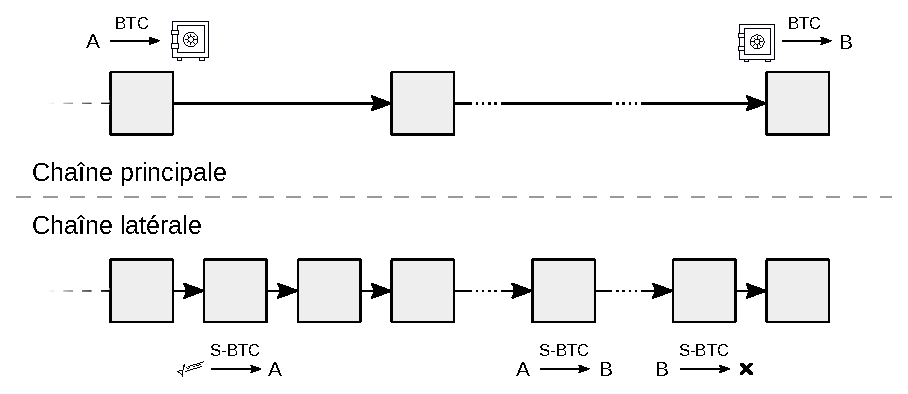
\includegraphics[scale=0.7]{img/sidechain-two-way-peg.eps}
  \caption{Chaîne latérale~: dépôt, transfert et retrait.}
  \label{fig:sidechain-two-way-peg}
\end{figure}

% Mécanisme de consensus
Le second aspect concerne la confirmation des transactions sur la chaîne latérale, et ici les options sont plus variées. Le consensus peut reposer sur le minage combiné, auquel cas c'est le travail de la chaîne principale qui est utilisé. Il peut se fonder sur la preuve d'enjeu, auquel cas c'est l'unité de la chaîne principale qui est impliquée. Ou il peut recourir à une fédération se mettant d'accord grâce à un algorithme BFT classique, auquel cas c'est l'appartenance à cette fédération qui importe (preuve d'autorité).

% Deux chaînes latérales sur BTC
Cette vision s'est concrétisée avec le lancement sur BTC de deux chaînes latérales distinctes en 2018. La première était RSK (aussi appelée Rootstock), qui a été lancée par Sergio Lerner en janvier de cette année-là et qui était focalisée sur l'exécution d'une machine virtuelle Turing-complète s'approchant de celle d'Ethereum. La seconde était Liquid, qui était la mise en œuvre du modèle Elements développé par Blockstream et dont le but primaire était de faciliter les transactions entre les différents acteurs financiers du secteur, dont notamment les plateformes d'échange. Dans Liquid, la sécurité repose sur une fédération de fonctionnaires qui assurent les deux rôles~: ils maintiennent l'ancrage du L-BTC en tant que gardiens (\eng{watchmen}) et participent au consensus de la chaîne en tant que signataires de blocs (\eng{blocksigners}). RSK allie le minage combiné et une fédération de «~notaires~» pour assurer à la fois l'ancrage du RBTC et le traitement des transactions.

% Risques
Les deux chaînes latérales n'ont cependant pas réussi à attirer une activité significative au fil des années, en raison des risques liés. En effet, utiliser ces chaînes requiert toujours une forme de confiance qui, bien que réduite au possible, reste bien présente. Un exemple malheureux d'une sidechain qui a mal tourné est celui de la chaîne latérale SmartBCH de Bitcoin Cash, où la société qui gérait le plus gros pont entre les deux chaînes, CoinFLEX, a fait faillite et n'a pas été en mesure de rembourser les utilisateurs\pagenote{«~la chaîne latérale SmartBCH de Bitcoin Cash~»~: CheapLightning, \eng{The Resolution of the smartBCH Experiment}, 2 août 2022~: \url{https://read.cash/@CheapLightning/the-resolution-of-the-smartbch-experiment-b06eb075}.}.

% --- Drivechain ---

Pour répondre à ces inconvénients et réduire la confiance impliquée, un protocole plus avancé a été élaboré par le chercheur Paul Sztorc depuis novembre 2015~: Drivechain\footnote{Paul Sztorc, \eng{Drivechain - The Simple Two Way Peg}, 24 novembre 2015~: \url{https://www.truthcoin.info/blog/drivechain/}.}. Comme son nom l'indique (\eng{drive chain} signifie chaîne de transmission), il s'agit d'une véritable machine de création et de gestion de chaînes latérales.

% Ancrage bilatéral est confié aux mineurs
La caractéristique principale de Drivechain est que l'ancrage bilatéral est confié aux mineurs, grâce au dépôt fiduciaire par taux de hachage (\eng{hashrate escrow}) défini dans le BIP-300\pagenote{«~BIP-300~»~: Paul Sztorc, CryptAxe, \eng{BIP-300: Hashrate Escrows}, 23 mai 2017~: \url{https://github.com/bitcoin/bips/blob/master/bip-0300.mediawiki}.}. Durant chaque période de six mois (26~300~blocs), les mineurs votent pour la transaction de retrait de la chaîne latérale distribuant les fonds aux utilisateurs en ayant fait la requête. La transparence et la lenteur de ces transactions permettent à l'ensemble des commerçants de la chaîne principale de les auditer. Les transferts courants, plus rapides, se font par des échanges atomiques ou par des services centralisés.

% Minage combiné « aveugle »
La validation des transactions sur la chaîne latérale utilisant Drivechain peut être assurée par n'importe quel algorithme de consensus. Mais le plus naturel est d'utiliser le minage combiné. C'est pourquoi le projet Drivechain contient également la proposition du minage combiné «~aveugle~» (BIP-301\pagenote{«~BIP-301~»~: Paul Sztorc, CryptAxe, \eng{BIP-301: Blind Merged Mining}, 23 juillet 2019~: \url{https://github.com/bitcoin/bips/blob/master/bip-0301.mediawiki}.}), une technique permettant aux mineurs de la chaîne principale de déléguer automatiquement la validation d'une chaîne latérale à autrui contre une rémunération. Le validateur gagne la différence entre le revenu de la chaîne latérale et l'achat du «~droit de trouver un bloc~». Ceci a pour effet de ne pas obliger les mineurs à gérer les chaînes latérales tout en touchant une partie de leur revenu. % Centralisation du minage à cause du minage combiné ?

% Inconvénients
Drivechain est un concept astucieux qui aurait pour avantage de pleinement réaliser la vision de Blockstream de 2014. Cependant, il présente un inconvénient majeur~: le modèle de sécurité de son ancrage bilatéral. Celui-ci repose en effet sur le recours éventuel à un soft fork réalisé par les commerçants dans le but de corriger une transaction de retrait frauduleuse, qui serait par exemple le fait de mineurs malintentionnés cherchant à voler l'argent du dépôt fiduciaire. Il se fonde donc sur la propension des commerçants à suivre l'activité de la chaîne latérale en question d'une part, et à procéder à une modification du protocole pour geler la transaction incriminée d'autre part. C'est pourquoi cette proposition est, encore aujourd'hui en 2023, largement disputée.

\section*{Le réseau Lightning}
\addcontentsline{toc}{section}{Le réseau Lightning}

% --- Réseau Lightning ---

% Présentation
Le réseau Lightning, ou \eng{Lightning Network} en anglais, est un concept de réseau de canaux de paiements bidirectionnels. Celui-ci a été présenté pour la première fois le 23 février 2015 par Joseph Poon et Thaddeus Dryja lors d'un séminaire de développeurs Bitcoin à San Francisco\footnote{Taariq Lewis, \eng{SF Bitcoin Devs Seminar: Scaling Bitcoin to Billions of Transactions Per Day}, 5 mars 2015~: \url{https://www.youtube.com/watch?v=8zVzw912wPo}.}. À l'époque, des propositions concurrentes basées sur des idées similaires existaient comme Amiko Pay (conceptualisé par Corné Plooy), Impulse (développé par Jeff Garzik pour Bitpay) et Ström (imaginé par la start-up Strawpay), mais Lightning est rapidement devenu dominant. En 2023, il s'agissait de la solution favorisée par les utilisateurs de BTC pour effectuer davantage de transferts, si bien que le sigle LNP/BP a émergé pour désigner l'ensemble des protocoles intervenant dans le passage en surcouche (à l'instar de TCP/IP vis-à-vis d'Internet)\pagenote{«~le sigle LNP/BP a émergé pour désigner l'ensemble des protocoles intervenant dans le passage en surcouche~»~: Giacomo Zucco, \eng{LNP/BP: A gentle introduction}, 21 juillet 2020, archive~: \url{https://web.archive.org/web/20200820123506/https://alzashop.com/lnp-bp-lightning-netowrk-and-bitcoin-protocols}.}.

% Canaux de paiement
L'infrastructure du réseau Lighning repose sur des canaux de paiement qui sont ouverts et fermés entre des participants. Un canal de paiement est, comme décrit dans le chapitre~\ref{ch:contrats}, un ensemble de contrats autonomes qui permet à deux personnes d'effectuer des paiements répétés de manière sûre et instantanée à partir de liquidités préalablement bloquées. L'utilisation d'un canal est par conséquent limitée par sa capacité, c'est-à-dire la somme des deux soldes des acteurs concernés.

% Fonctionnement de Lightning
Le principe du réseau Lightning est de router les paiements au travers de ces canaux par l'intermédiaire de HTLC, qui sont des contrats d'engagement plus complexes permettant de mettre à jour les canaux concernés\footnote{En pratique, ces HTLC sont souvent aussi utilisés pour mettre à jour les canaux directement, afin de simplifier la mise en œuvre et d'améliorer la confidentialité. -- Voir Andreas M. Antonopoulos, Olaoluwa Osuntokun, René Pickhardt, «~Routing on a Network of Payment Channels~», in \eng{Mastering the Lightning Network: A Second Layer Blockchain Protocol for Instant Bitcoin Payments}, O'Reilly Media, 2022, pp.~185--207.}. Un paiement transite sur le réseau moyennant des frais minimes qui vont aux nœuds le relayant. Le réseau Lightning est donc semblable à un boulier, dont les tiges sont des canaux et dont les boules sont les satoshis qui transitent d'un côté ou de l'autre des canaux, comme on peut le voir sur la figure~\ref{fig:lightning-network-abacus}.

\begin{figure}[ht]
  \centering
  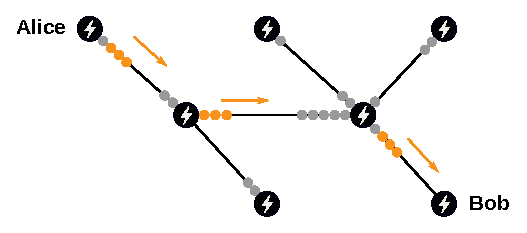
\includegraphics[scale=1.1]{img/lightning-network-abacus.eps}
  \caption{Paiement de 3~mBTC sur le réseau Lightning.}
  \label{fig:lightning-network-abacus}
\end{figure}

% Avantages de Lightning
Ce fonctionnement offre la possibilité de réaliser des paiements quasi instantanés et peu chers. Il permet de faire plus de transferts en bitcoins sans réaliser davantage de transactions sur la chaîne et sans déléguer explicitement la gestion des fonds à un tiers. De plus, le modèle conserve toute la programmabilité de Bitcoin et ouvre le champ des possibles quant à l'utilisation monétaire sur Internet.

% Inconvénients de Lightning
Toutefois, l'apport de Lightning est à nuancer car il n'est pas exempt de défauts. D'abord, il hérite des inconvénients liés au modèle des canaux de paiement où, dans le cas du protocole de Poon-Dryja, une erreur peut mener à la perte des fonds. Puis, les contraintes liées à la capacité et au routage créent nécessairement une tendance à la centralisation, notamment par l'émergence de ce qu'on appelle les \eng{Lightning Service Providers}, ce qui pourrait mener à l'installation d'une certaine censure. Ensuite, contrairement aux idées reçues, la confidentialité sur Lightning est faible, les paiements se faisant entre des clés publiques identifiées et transitant par des intermédiaires. Enfin, le réseau est soumis au niveau des frais sur la chaîne principale, ces derniers étant nécessaires au règlement des contrats, ce qui limite la capacité transactionnelle supplémentaire apportée.

% Pertinence et développement
Le réseau Lightning est donc adapté pour traiter les paiements du quotidien et les micropaiements, ne nécessitant pas forcément la confidentialité et la résistance à la censure offertes par la chaîne de blocs, à partir de canaux bien pourvus et régulièrement réapprovisionnés. Il a été mis en œuvre à partir de janvier 2018, principalement en surcouche de BTC, et s'est développé considérablement depuis, tant d'un point de vue technique qu'économique. Trois implémentations logicielles ont été maintenues par trois entités différentes (lnd par Lightning Labs, c-lightning par Blockstream, eclair par ACINQ) et un système de standards techniques (appelés \eng{Bases of Lightning Technology} ou BOLT) a fini par émerger. Du côté économique, le réseau a rencontré un certain succès en attirant les capitaux et, en novembre 2023, une capacité totale de 5~400~BTC, équivalant à environ 200 millions de dollars, était réservée pour fournir de la liquidité pour les paiements\pagenote{«~en novembre 2023, une capacité totale de 5~400~BTC, équivalant à environ 200 millions de dollars~»~: \url{https://bitcoinvisuals.com/ln-capacity}.}.

\section*{Les banques chaumiennes de Fedimint}
\addcontentsline{toc}{section}{Les banques chaumiennes de Fedimint}

Une autre proposition est Fedimint\footnote{Le fonctionnement de Fedimint est décrit dans la documentation présente sur le site web~: \url{https://fedimint.org/docs/intro}.}, qui est un protocole de garde et d'échange confidentiel de bitcoins dans un contexte communautaire. D'un point de vue technique, il s'agit de confier la garde des bitcoins à une fédération et d'échanger des billets chaumiens (eCash) émis par ladite fédération. Ce fonctionnement explique le nom du protocole, qui est une abréviation approximative de \eng{Federated Chaumian Mint} («~monnaierie chaumienne fédérée~» en français).

% Origine
Fedimint a été imaginé par le cypherpunk Eric Sirion au cours de l'année 2021 et implémenté sous forme minimale sous le nom de MiniMint\pagenote{«~MiniMint~»~: Kiara Bickers, \eng{Blockstream Sponsors Federated E-Cash as a Bitcoin Scaling Technology}, 26 octobre 2021~: \url{https://medium.com/blockstream/blockstream-sponsors-federated-e-cash-as-a-bitcoin-scaling-technology-637ba05de7b3}.}. Sirion a été doublement inspiré par les tentatives d'appliquer eCash en surcouche de Bitcoin comme SCRIT\pagenote{«~SCRIT~»~: \url{https://github.com/scritcash/scrit-whitepaper/blob/master/scrit-whitepaper.pdf}.} et par les approches communautaires telles que Bitcoin Beach au Salvador. La première transaction d'une fédération Fedimint a eu lieu le 28 septembre 2022 durant le Hackers Congress de Paralelni Polis.

% --- eCash ---

La première composante de Fedimint est la banque chaumienne qui est gérée par la fédération. Celle-ci utilise le procédé de signature aveugle de David Chaum pour émettre des certificats adossés à un certain montant de satoshis, qui peut être récupéré à tout moment sur la chaîne ou sur le réseau Lightning. Cette composante assure la confidentialité financière partielle des participants~: la banque n'a pas connaissance des échanges réalisés par les clients, mais son rôle de prévention de la double dépense exige qu'elle voie les revenus des commerçants\footnote{Le fonctionnement technique des systèmes chaumiens a été décrit dans la section «~eCash~: l'argent liquide chaumien~» du chapitre~\ref{ch:cybermonnaie}.}.

% eCash et Bitcoin
L'idée d'utiliser eCash en surcouche de Bitcoin n'est pas une idée nouvelle. Elle a été proposée et implémentée pour la première fois le 17 août 2010, par un individu intervenant sous le pseudonyme fellowtraveller sur le forum de Bitcoin sous la forme de son projet Open Transactions\pagenote{«~Open Transactions~»~: fellowtraveler, \eng{Open Transactions: untraceable digital cash}, \wtime{17/08/2010 20:58:05 UTC}~: \url{https://bitcointalk.org/index.php?topic=847.msg9976\#msg9976}.}. Le projet ne s'est jamais imposé, car le besoin ne se faisait pas ressentir et le système était probablement trop complexe. Cependant, l'idée est revenue timidement sur les devants de la scène au cours du débat sur la scalabilité avec la proposition des «~certificats aveugles au porteur\pagenote{«~certificats aveugles au porteur~»~: Michael Marquardt (Theymos), \eng{Blinded bearer certificates}, \wtime{28/12/2016 21:44:24}~: \url{https://www.reddit.com/r/Bitcoin/comments/5ksu3o/blinded_bearer_certificates/}.}~» de Theymos (administrateur du subreddit r/Bitcoin et du forum Bitcointalk) en décembre 2016. Elle a également été reprise en 2019 par Frank Braun et Jonathan Logan (coanimateurs du podcast Cypherpunk Bitstream) au moyen de SCRIT, un projet de système chaumien fédéré dont le nom est l'acronyme de «~\eng{Secure, Confidential, Reliable, Instant Transactions}~». Le dernier projet en date d'une mise en œuvre d'un système chaumien centralisé est Cashu, un protocole développé en 2022 par le développeur callebtc, qui permet la création et l'échange de certificats-bitcoin en surcouche de Lightning et de nouveaux jetons\pagenote{«~Cashu~»~: callebtc sur Twitter, \wtime{14/09/2022 09:47 UTC}~: \url{https://twitter.com/callebtc/status/1569986110272540674}.}.

% --- Approche communautaire ---

L'intérêt de Fedimint, tout comme son prédécesseur SCRIT, est de décentraliser la garde de bitcoins. Pour ce faire, il combine le système chaumien avec une approche dite «~communautaire~», consistant à déployer une banque gérée par les membres de confiance d'une communauté locale.

% Bitcoin Beach
Cette approche a été illustrée par l'expérience de Bitcoin Beach, un projet de développement économique durable autour de la plage d'El Zonte au Salvador. Une banque communautaire a ainsi vu le jour en 2020 et permet depuis lors aux locaux d'échanger des bitcoins de façon sûre et fiable, par le biais du Bitcoin Beach Wallet (devenu Blink) développé par Galoy. C'est cette expérience qui a inspiré l'adoption du cours légal à l'échelle nationale en septembre 2021.

% Fédération
La deuxième composante de Fedimint est donc une fédération, semblable aux fédérations des chaînes latérales comme Liquid ou RSK, mais composée de personnes de confiance qui possèdent les capacités techniques nécessaires à la gestion d'un nœud. Les membres de cette fédération, appelés gardiens, sont responsables de la mise en place de l'infrastructure et se chargent de conserver les fonds des utilisateurs et d'assurer le bon fonctionnement de la banque chaumienne. Ils se coordonnent en utilisant un algorithme de consensus classique (appelé HBBFT\pagenote{«~HBBFT~»~: Il s'agit du sigle de \eng{Honey Badger Byzantine Fault Tolerant}.}) qui, comme tous les algorithmes de ce type, demande un minimum de 66~\% d'acteurs honnêtes pour fonctionner. % Cette composante assure la garde communautaire des fonds.

% Risques
L'emploi de cette fédération représente un compromis technique évident entre la propriété entière des fonds et sa délégation auprès d'un acteur unique. Ce compromis apporte des avantages majeurs au niveau des frais de traitement des transactions et de la facilité d'utilisation, mais engendre également des risques importants. Ceux-ci sont le risque de garde (la fédération peut voler ou perdre des fonds), le risque d'émission frauduleuse (elle peut émettre plus de certificats qu'elle n'a de bitcoins), le risque de censure (elle peut refuser de valider une transaction) et le risque réglementaire (la fédération peut être saisie et fermée sur décision étatique).

% Objectif de Fedimint : prendre le rôle des applications dépositaires
Tout ceci fait que Fedimint ne peut pas être conçue comme une solution de scalabilité, mais comme une proposition de remplacement des applications dépositaires. L'objectif de Fedimint est d'améliorer la garde de bitcoins en la décentralisant et en accroissant la confidentialité des échanges internes. Son caractère local doit permettre d'échapper aux réglementations financières, et ainsi de ne pas subir le sort réservé aux banques classiques.

% La troisième composante est le système d'échanges (atomiques) avec le réseau Lightning. Chaque échange a lieu entre la fédération et un utilisateur par un HTLC. Cela permet la mise en place de passerelles Lightning, qui s'assurent du transfert des fonds depuis ou vers Lightning ou d'autres communautés fédérées pour une aisance d'utilisation optimale. Cette composante assure l'interopérabilité à l'échelle globale entre les communautés.

\section*{Le passage à l'échelle par substitution}
\addcontentsline{toc}{section}{Le passage à l'échelle par substitution}

% Limites des surcouches
Le passage en surcouche est une manière correcte d'accroître le volume économique lié à une chaîne donnée sans trop affecter ses caractéristiques premières. Néanmoins, cette approche présente aussi des limites~: non seulement les différentes surcouches ont leurs défauts propres, mais surtout elles reposent en dernier lieu sur le règlement réalisé sur la chaîne de blocs, dont la capacité est limitée. Par conséquent, le plancher d'utilité n'est pas supprimé par le passage en surcouche et on ne peut ainsi pas voir ce dernier comme un moyen miraculeux de traiter une infinité de transactions.

% Effet de substitution
La plage de valeurs desservie par un système cryptomonétaire donné a pour effet de créer une demande pour des systèmes de substitution plus à même d'assurer le transfert hors de cette plage. Un système dont le niveau de frais est élevé laisse la voie libre à l'utilisation d'un système moins sûr mais moins cher, permettant le traitement des plus petites transactions. À l'inverse, un système dont le niveau de sécurité est faible favorise l'émergence d'un système plus cher mais aussi plus sûr, autorisant les plus gros transferts. Il existe de ce fait une certaine complémentarité entre les différentes mises en œuvre de Bitcoin qui permettent de gérer l'intégralité de l'activité transactionnelle émanant des utilisateurs\footnote{Eric Voskuil, «~Principe de substitution~», in \emph{Cryptoéconomie~: Principes fondamentaux de Bitcoin}, Amazon KDP, 2022, pp.~315--316.}.

% Complémentarité de l'or et de l'argent
Au cours de l'histoire, une telle complémentarité s'est manifestée par l'utilisation de plusieurs métaux précieux comme base monétaire. L'or ne pouvait pas permettre de couvrir toutes les plages de valeurs~: celui-ci était adapté au transfert de grosses sommes, chose pour laquelle il a été sélectionné comme monnaie de réserve mondiale, mais pas à l'échange de petite monnaie. C'est pour remplir ce dernier rôle complémentaire que l'argent, et d'autres métaux moins précieux comme le cuivre, ont été utilisés. L'argent, mot qu'on utilise encore aujourd'hui en français comme synonyme de monnaie, était la monnaie du quotidien tandis que l'or servait essentiellement aux règlements plus onéreux.

% Bimétallisme
Cet aspect bimétallique (voire trimétallique) de la monnaie a perduré pendant des siècles, de la Haute Antiquité jusqu'au \textsc{xix}\ieme{} siècle. Il était reconnu par les pouvoirs publics qui définissaient leur monnaie comme un poids en or ou en argent, et frappaient des pièces d'or et d'argent en décrétant un taux de change selon le ratio or-argent du marché. On constate d'ailleurs que ce ratio or-argent a été relativement stable au cours de l'histoire en variant entre 10 et 18\pagenote{«~ce ratio or-argent a été relativement stable au cours de l'histoire en variant entre 10 et 18~»~: William Jacob, \eng{An Historical Inquiry Into the Production and Consumption of the Precious Metals}, 1831.}, ce qui confirme le rôle monétaire de l'argent aux côtés de l'or.

% Démonétisation de l'argent
Toutefois, avec l'émergence de l'étalon-or et la disparition du bimétallisme à la fin du \textsc{xix}\ieme{}~siècle, l'argent a peu à peu perdu son rôle monétaire pour être remplacé par la monnaie papier, dans un premier temps adossée à l'or, bien plus commode pour effectuer des échanges. Le ratio a augmenté en conséquence et est passé de 15,5 en 1870 à 80 aujourd'hui, ce qui correspond à une perte de valeur de l'argent de plus de 80~\% par rapport à l'or.

% Litecoin est à l'argent ce que Bitcoin est à l'or
L'analogie avec les métaux précieux est éclairante. Puisque la version principale de Bitcoin (BTC) n'est pas adaptée pour traiter les transferts de plus petite valeur, il s'ensuit que ces transferts potentiels sont réalisés au moyen d'une monnaie de substitution (de la cryptomonnaie, de la monnaie fiat liquide, du crédit déplacé par des services bancaires permissifs, etc.) voire ne sont pas traités du tout. Litecoin, dont la principale narration est qu'il s'agirait d'un argent numérique au même titre que Bitcoin serait un or numérique, répond tout à fait à cette demande. Il était ainsi présenté dès son lancement comme une «~version allégée de Bitcoin~» ayant pour but d'être «~à l'argent ce que Bitcoin est à l'or\footnote{Charlie Lee, \eng{Re: [ANN] Litecoin - a lite version of Bitcoin. Be ready when is launches!}, \wtime{09/10/2011 06:14:28 UTC}~: \url{https://bitcointalk.org/index.php?topic=47417.msg564414\#msg564414}.}~». Cette désignation ne provient pas tant du fait qu'il y a quatre fois plus de litecoins que de bitcoins, ce qui n'a aucune incidence sur le système, mais plutôt du fait que la capacité transactionnelle maximale de LTC est quatre fois plus grande, ce qui amoindrit la sécurité potentielle du système. Cette analyse vaut également pour Bitcoin Cash à une échelle encore plus grande.

% Services de change, atomic swaps
Dans cette vision, les mises en œuvre alternatives de Bitcoin serviraient à traiter toutes les transactions, au prix de nécessaires transferts entre les chaînes. Ces derniers seraient assurés par des services de change centralisés ou par des systèmes d'échanges atomiques basés sur des carnets d'ordres publics. Cette solution, bien qu'imparfaite, serait tout à fait naturelle et est d'ailleurs déjà pratiquée aujourd'hui.

% Extensivité : confidentialité, programmabilité, noms de domaine
L'extensivité est également concernée par cet effet. Le coût technique d'une utilisation complexe de Bitcoin peut être compensé par des systèmes de substitution de moindre qualité. La confidentialité à bas coût peut être assurée par Monero et la programmabilité simplifiée par Ethereum Classic par exemple. Comme le remarquait très justement Satoshi Nakamoto en décembre 2010, à propos de la pertinence de BitDNS (le futur Namecoin)~:

\begin{quote}
«~Le fait de rassembler tous les systèmes de quorum par preuve de travail dans une seule base de données ne passe pas à l'échelle. Bitcoin et BitDNS peuvent être utilisés séparément. [...] Les réseaux ont besoin d'avoir des destins différents. Les utilisateurs de BitDNS pourraient être extrêmement tolérants vis-à-vis de l'ajout de fonctionnalités permettant de traiter des données volumineuses, puisque peu de registraires de noms de domaine seraient nécessaires, tandis que les utilisateurs de Bitcoin pourraient devenir de plus en plus sectaires à propos de la limitation de la taille de la chaîne, pour que son accès reste facile pour beaucoup d'utilisateurs et pour les petits appareils\footnote{Satoshi Nakamoto, \eng{Re: BitDNS and Generalizing Bitcoin}, \wtime{10/12/2010, 17:29:28}~: \url{https://bitcointalk.org/index.php?topic=1790.msg28917\#msg28917}.}.~»
\end{quote}

\vspace{-2em}
\section*{Trois types de compromis}
\addcontentsline{toc}{section}{Trois types de compromis}

La scalabilité de Bitcoin est un sujet complexe. Contrairement à ce qui est parfois affirmé, un système donné est très peu scalable. Sa capacité à passer à l'échelle ne peut être améliorée qu'au moyen d'optimisations logicielles, matérielles ou algorithmiques. Le gain en performance sur la chaîne se fait la plupart du temps au prix d'un compromis direct, avec l'augmentation de la limite de capacité transactionnelle, ou indirect, avec l'altération du modèle de sécurité.

C'est la raison de l'existence du passage en surcouche, qui consiste à déporter une partie des transferts économiques vers des protocoles ouverts et décentralisés, préservant partiellement les propriétés de Bitcoin et reposant sur le règlement des litiges sur la chaîne. Dans cette démarche, le compromis de sécurité est partiel et limité dans le temps, contrairement au cas de l'augmentation de capacité transactionnelle où il est total et persistant. Le passage de surcouche s'est développé sur BTC au cours du temps par le biais des chaînes latérales, proposées en 2014 et mises en œuvre en 2018, du réseau Lightning, proposé en 2015 et déployé depuis 2018, et de Fedimint, proposé en 2021.

L'autre alternative est le passage à l'échelle par substitution, qui consiste, en substance, à déplacer les transactions les moins à risque vers des substituts de moins bonne qualité, c'est-à-dire des mises en œuvre moins sécurisées du concept Bitcoin. Cet effet s'est réellement manifesté pour la première fois en 2017 avec les premières congestions du réseau BTC et la hausse de la demande pour des contrats autonomes statiques (Ethereum), qui se sont notamment accompagnées d'une baisse de la dominance économique de la version principale de Bitcoin. Les maximalistes ont tendance à prétendre que le passage en surcouche permet de traiter l'ensemble des utilisations pertinentes de Bitcoin, mais, jusqu'à preuve du contraire, ce n'est pas le cas.
